% SC4013 --- Chapter 1: OWASP Top 10 Overview and Risk (0->100 ground-up)
\chapter{OWASP Top 10: Mapping the Battlefield}\label{ch:owasp}

\begin{quote}
\emph{``If you know the enemy and know yourself, you need not fear the result of a hundred battles.''} --- Sun Tzu. The OWASP Top 10 is our map of where web applications most often lose those battles.
\end{quote}

\noindent\fbox{\parbox{\dimexpr\linewidth-2\fboxsep-2\fboxrule}{%
\textbf{From zero: no security background assumed.} We start from an everyday analogy---a building with doors, windows and tenants---and build the language of vulnerabilities, exploits and risk from scratch. Every term is defined when first used. This chapter is the atlas for the rest of the book.}}
\vspace{0.4em}

\section*{Learning Outcomes}
After this chapter you will be able to:
\begin{enumerate}[label=(L\arabic*)]
    \item explain what OWASP is and why community consensus matters;
    \item name and summarise the OWASP Top 10 (2021) categories with examples;
    \item compute risk as $\text{Likelihood}\times\text{Impact}$ and apply the OWASP Risk Rating;
    \item sketch an application's attack surface from its data-flow diagram;
    \item argue why ``Top 10'' is a starting checklist, not a complete security programme.
\end{enumerate}

% ============================================================
\section{What Is OWASP and Why a Top 10?}\label{sec:what-is-owasp}
Picture a city where every landlord secures their building differently. One installs deadbolts; another leaves the service entrance propped open. Burglars learn which mistakes recur most often and target them at scale. Web security has the same dynamic, except the city is the Internet and the buildings are applications.

The \emph{Open Worldwide Application Security Project} (OWASP) is a non-profit community that collects real breach data, practitioner surveys, and vendor findings, then distills them into guidance anyone can use. Its flagship list, the \emph{OWASP Top 10}, answers one question: \emph{which ten weakness classes cause the most real-world harm right now?} It is not a standard, not a certification, and not exhaustive---it is a prioritised awareness document updated every few years (2004, 2007, 2010, 2013, 2017, 2021).

Two ideas make it powerful. First, \emph{consensus}: thousands of organisations contribute data, so the list reflects what attackers actually exploit, not what academics find elegant. Second, \emph{mapping}: each category links to Common Weakness Enumeration (CWE) entries and testing guides, so a team can move from name to concrete check.

\begin{definition}[Vulnerability, exploit, risk]\label{def:ver}
A \emph{vulnerability} is a flaw that violates a security property. An \emph{exploit} is a concrete input or sequence that triggers the flaw. \emph{Risk} combines how likely an exploit is and how much damage success would cause. The Top 10 ranks by approximate risk, not raw bug count.
\end{definition}

\begin{example}[From bug to risk]
A search box that reflects user input without escaping is a vulnerability (Cross-Site Scripting). Sending \texttt{<script>alert(1)</script>} is an exploit. If that page is the admin console, the risk is high; if it is an isolated static page, the risk is lower. Same bug class, different risk.
\end{example}

% ============================================================
\section{The OWASP Top 10 (2021) at a Glance}\label{sec:top10}
The 2021 edition reshaped the list around modern architectures (APIs, supply chains, cloud). Memorise the shape, not just the acronyms:

\begin{center}
\small
\begin{tabular}{clp{7.5cm}c}
\toprule
\# & Category & What it means (plain language) & CWE family\\
\midrule
A01 & Broken Access Control & Users can act outside their permissions (IDOR, path traversal) & 352/639\\
A02 & Cryptographic Failures & Secrets or data exposed due to weak/absent crypto & 311/327\\
A03 & Injection & Untrusted input executed as code or query & 77/89\\
A04 & Insecure Design & Security was never part of the design (no threat model) & 209/657\\
A05 & Security Misconfiguration & Defaults, open S3 buckets, verbose errors & 16/611\\
A06 & Vulnerable Components & Using libraries with known CVEs & 1104\\
A07 & Auth Failures & Broken login, session, or credential recovery & 287/384\\
A08 & Data Integrity Failures & Untrusted updates, deserialisation, CI/CD poisoning & 829/502\\
A09 & Logging \& Monitoring Failures & Breaches undetected for months & 778\\
A10 & SSRF & Server tricked into fetching attacker-chosen URLs & 918\\
\bottomrule
\end{tabular}
\end{center}

\begin{figure}[h]\centering
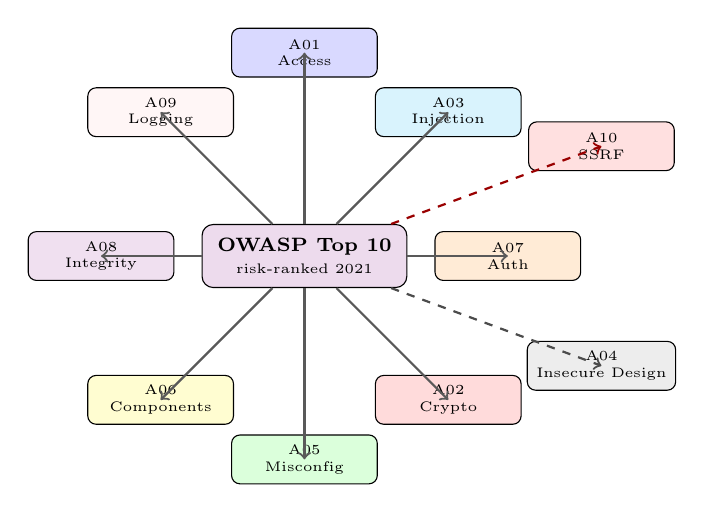
\begin{tikzpicture}[scale=0.82, every node/.style={font=\scriptsize}]
  % centre
  \node[draw,fill=violet!14,rounded corners=4pt,minimum width=2.6cm,minimum height=0.8cm,align=center] (c) at (0,0) {\textbf{OWASP Top 10}\\ \tiny risk-ranked 2021};
  % outer ring nodes
  \foreach \a/\col/\txt in {
    90/blue!15/A01\\Access,
    45/cyan!15/A03\\Injection,
    0/orange!16/A07\\Auth,
    -45/red!14/A02\\Crypto,
    -90/green!14/A05\\Misconfig,
    -135/yellow!18/A06\\Components,
    180/violet!12/A08\\Integrity,
    135/pink!14/A09\\Logging} {
    \node[draw,fill=\col,rounded corners=3pt,minimum width=1.85cm,minimum height=0.62cm,align=center,font=\tiny] at (\a:3.15) {\txt};
    \draw[->,thick,gray!70!black] (c) -- (\a:3.15);
  }
  % SSRF + Design as side callouts
  \node[draw,fill=red!12,rounded corners=3pt,minimum width=1.85cm,minimum height=0.62cm,align=center,font=\tiny] at (4.6,1.7) {A10\\SSRF};
  \node[draw,fill=gray!14,rounded corners=3pt,minimum width=1.85cm,minimum height=0.62cm,align=center,font=\tiny] at (4.6,-1.7) {A04\\Insecure Design};
  \draw[->,thick,red!60!black,dashed] (c) -- (4.6,1.7);
  \draw[->,thick,gray!60!black,dashed] (c) -- (4.6,-1.7);
\end{tikzpicture}
\caption{Eight perennial + two modern categories (A04 Design and A10 SSRF, dashed) radiate from the central idea: the Top 10 is a risk-ranked map, not a checklist to ``complete.'' Colour groups injection-adjacent (blue/cyan), access/auth (orange/red), and supply-chain (yellow/violet).}
\label{fig:owasp-wheel}
\end{figure}

Three design lessons stand out. \emph{A04 Insecure Design} is new: it says some flaws cannot be patched---you must design differently. \emph{A06 Vulnerable Components} reminds us that \texttt{npm install} is a trust decision: every dependency extends your attack surface. \emph{A10 SSRF} reflects cloud reality: when the server can fetch URLs, the attacker can pivot inside the private network.

\begin{remark}[Not a ceiling]
Passing ``Top 10 checks'' does not mean secure. Business-logic flaws, race conditions and denial-of-service rarely make the list but still rupture systems. Use the list to prioritise, then go deeper (Ch.~3--8).
\end{remark}

% ============================================================
\section{\texorpdfstring{Risk: Why We Rank by Likelihood $\times$ Impact}{Risk: Why We Rank by Likelihood x Impact}}\label{sec:risk}
A long bug list is useless without ranking. OWASP borrows a simple model:

\begin{equation}\label{eq:risk}
\text{Risk} = \text{Likelihood} \times \text{Impact}
\end{equation}
where Likelihood itself splits into \emph{threat-agent factors} (skill, motive, opportunity, population size) and \emph{vulnerability factors} (ease of discovery, ease of exploit, awareness, intrusion detection). Impact splits into \emph{technical impact} (confidentiality, integrity, availability, accountability loss) and \emph{business impact} (financial, reputation, compliance, privacy).

\begin{figure}[h]\centering
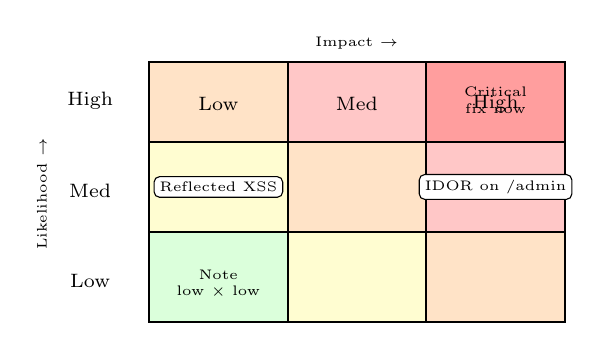
\begin{tikzpicture}[scale=0.88, every node/.style={font=\scriptsize}]
  \fill[green!14] (0,0) rectangle (2.0,1.3);
  \fill[yellow!18] (2.0,0) rectangle (4.0,1.3);
  \fill[orange!22] (4.0,0) rectangle (6.0,1.3);
  \fill[yellow!18] (0,1.3) rectangle (2.0,2.6);
  \fill[orange!22] (2.0,1.3) rectangle (4.0,2.6);
  \fill[red!22] (4.0,1.3) rectangle (6.0,2.6);
  \fill[orange!22] (0,2.6) rectangle (2.0,3.75);
  \fill[red!22] (2.0,2.6) rectangle (4.0,3.75);
  \fill[red!38] (4.0,2.6) rectangle (6.0,3.75);
  \foreach \x/\lab in {0/Low,2.0/Med,4.0/High} \node at (\x+1.0,3.15) {\lab};
  \foreach \y/\lab in {0/Low,1.3/Med,2.6/High} \node at (-0.85,\y+0.6) {\lab};
  \node[font=\tiny,align=center] at (5.0,3.2) {Critical\\fix now};
  \node[font=\tiny,align=center] at (1.0,0.55) {Note\\low $\times$ low};
  \draw[thick,black] (0,0) rectangle (6.0,3.75);
  \draw[thick] (2.0,0)--(2.0,3.75); \draw[thick] (4.0,0)--(4.0,3.75);
  \draw[thick] (0,1.3)--(6.0,1.3); \draw[thick] (0,2.6)--(6.0,2.6);
  \node[font=\tiny,above] at (3.0,3.80) {Impact $\to$}; \node[font=\tiny,rotate=90] at (-1.55,1.85) {Likelihood $\to$};
  % annotate example
  \node[draw,fill=white,rounded corners=2pt,inner sep=2pt,font=\tiny] at (5.0,1.95) {IDOR on /admin};
  \node[draw,fill=white,rounded corners=2pt,inner sep=2pt,font=\tiny] at (1.0,1.95) {Reflected XSS};
\end{tikzpicture}
\caption{Risk heatmap (OWASP Risk Rating simplified). Colour deepens toward top-right where likely exploits meet severe impacts. An IDOR on an admin endpoint lands in the red zone; reflected XSS on a marketing page sits lower. Ranking drives where to spend engineering time.}
\label{fig:risk-heatmap}
\end{figure}

\begin{definition}[OWASP Risk Rating]\label{def:owasp-risk}
Score each factor $0$--$9$. Average the eight likelihood sub-factors into $L$, the four technical-impact factors into $I_T$, and the four business-impact factors into $I_B$, then $\text{Risk}_T=L\times I_T$ and $\text{Risk}_B=L\times I_B$. Map $0$--$3$ to Low, $3$--$6$ to Medium, $6$--$9$ to High/Critical. Teams fix top-right first.
\end{definition}

\begin{lstlisting}[language=Python]
# Simplified OWASP Risk Rating calculator
def owasp_risk(likelihood_factors, tech_impact, biz_impact):
    """Each arg is a list of 0-9 scores. Returns (tech_risk, biz_risk, band)."""
    L = sum(likelihood_factors) / len(likelihood_factors)
    IT = sum(tech_impact) / len(tech_impact)
    IB = sum(biz_impact) / len(biz_impact)
    tech_risk, biz_risk = L * IT, L * IB
    def band(s): return "Low" if s < 3 else "Medium" if s < 6 else "High"
    return round(tech_risk,1), round(biz_risk,1), band(max(tech_risk, biz_risk))

# Example: IDOR on /api/user/{id} with no auth check
print(owasp_risk([8,7,9,8,7,8,9,2], [9,9,7,7], [8,7,7,9]))
# -> (58.0, 56.5, 'High')  -- compare: reflected XSS may score ~20 'Medium'
\end{lstlisting}

A number never replaces judgement, but a shared scoring rubric stops the loudest voice from always winning prioritisation.

% ============================================================
\section{Attack Surface: Seeing What the Attacker Sees}\label{sec:surface}
An \emph{attack surface} is the sum of all points where an attacker can interact with the system and potentially cause harm: every endpoint, parameter, header, file upload, WebSocket, third-party callback, and debug flag left enabled.

\begin{figure}[h]\centering
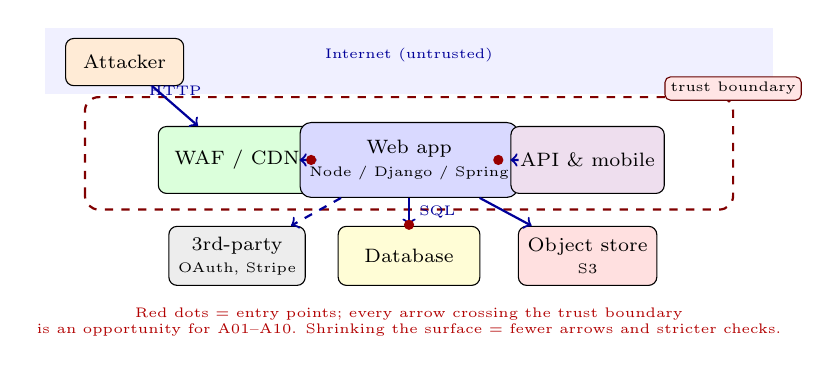
\begin{tikzpicture}[scale=0.84, every node/.style={font=\scriptsize}]
  % Internet
  \fill[blue!6] (-5.5,2.6) rectangle (5.5,3.6);
  \node[font=\tiny,blue!60!black] at (0,3.18) {Internet (untrusted)};
  \node[draw,fill=orange!16,rounded corners=3pt,minimum width=1.5cm,minimum height=0.6cm,align=center] (att) at (-4.3,3.08) {Attacker};
  % App
  \node[draw,fill=green!14,rounded corners=3pt,minimum width=2.0cm,minimum height=0.85cm,align=center] (waf) at (-2.6,1.6) {WAF / CDN};
  \node[draw,fill=blue!15,rounded corners=4pt,minimum width=2.2cm,minimum height=0.95cm,align=center] (web) at (0,1.6) {Web app\\ \tiny Node / Django / Spring};
  \node[draw,fill=violet!13,rounded corners=3pt,minimum width=1.7cm,minimum height=0.85cm,align=center] (api) at (2.7,1.6) {API \& mobile};
  \node[draw,fill=yellow!16,rounded corners=3pt,minimum width=1.8cm,minimum height=0.75cm,align=center] (db) at (0,0.15) {Database};
  \node[draw,fill=red!12,rounded corners=3pt,minimum width=1.7cm,minimum height=0.75cm,align=center] (store) at (2.7,0.15) {Object store\\ \tiny S3};
  \node[draw,fill=gray!14,rounded corners=3pt,minimum width=1.6cm,minimum height=0.75cm,align=center] (third) at (-2.6,0.15) {3rd-party\\ \tiny OAuth, Stripe};
  % Trust boundary
  \draw[thick,red!50!black,dashed,rounded corners=5pt] (-4.9,0.85) rectangle (4.9,2.55);
  \node[font=\tiny,fill=red!10,draw=red!40!black,rounded corners=2pt,inner sep=2pt] at (4.9,2.68) {trust boundary};
  % Flows
  \draw[->,thick,blue!60!black] (att) -- (waf) node[midway,above,font=\tiny] {HTTP};
  \draw[->,thick,blue!60!black] (waf) -- (web); \draw[->,thick,blue!60!black] (web) -- (api);
  \draw[->,thick,blue!60!black] (web) -- (db) node[midway,right,font=\tiny] {SQL};
  \draw[->,thick,blue!60!black] (web) -- (store); \draw[->,thick,blue!60!black,dashed] (web) -- (third);
  % Entry point dots
  \foreach \p in {(-1.48,1.6),(1.35,1.6),(0,0.62)} \fill[red!60!black] \p circle (2.2pt);
  \node[font=\tiny,red!70!black,align=center] at (0,-0.85) {Red dots = entry points; every arrow crossing the trust boundary\\is an opportunity for A01--A10. Shrinking the surface = fewer arrows and stricter checks.};
\end{tikzpicture}
\caption{Attack surface sketch for a typical web application. The dashed box is the trust boundary: everything outside is attacker-controlled. Each crossing is where input validation, authentication and authorisation must happen. Adding a feature (chat, upload, webhook) adds crossings.}
\label{fig:attack-surface}
\end{figure}

Shrinking the surface is the most durable defence: disable unused endpoints, enforce allow-lists on inputs (Ch.~3), and require authentication before any state-changing action (Ch.~2 and Ch.~4). A Top 10 category then becomes a lens for one kind of crossing: A03 Injection watches data that becomes code, A01 Access Control watches who may cross, A07 Authentication watches who they claim to be.

\begin{remark}[Checklists versus thinking]
The Top 10 is a mirror, not a finish line. New technologies (GraphQL, serverless, supply-chain) create new A04/A08/A10 variants before the next edition. Teams that internalise likelihood$\times$impact and draw their surface honestly will catch tomorrow's A11 before it is named.
\end{remark}

% ============================================================
\section{Exercises}\label{sec:ch01-exercises}
\begin{enumerate}[label=E1.\arabic*, leftmargin=*, itemsep=0.6em]
    \item \textbf{Mapping a breach.} Pick a public breach from the last two years. Map its root cause to one OWASP Top 10 (2021) category and one CWE. Identify one likelihood factor and one impact factor that made the risk High.
    \item \textbf{Risk scoring.} Score two endpoints with the simplified function in the listing: (a) unauthenticated \texttt{GET /api/backup.zip} and (b) reflected XSS on \texttt{/search?q=}. Choose your own 0--9 sub-scores, justify each, and compute the band. Does the ranking match intuition? Swap one factor and observe the change.
    \item \textbf{Attack surface enumeration.} Draw a data-flow diagram for a food-delivery app (customer app $\to$ API gateway $\to$ order service $\to$ DB plus courier app and payment webhook). Mark the trust boundary and list at least six entry points. For each, name the Top 10 category most relevant to that crossing.
    \item \textbf{A04 vs A05.} Contrast Insecure Design (A04) with Security Misconfiguration (A05) on a feature that lets users upload profile pictures. Give one example of each, explain why patching the A05 instance does not fix the A04 flaw, and propose a design-level mitigation for the latter.
    \item \textbf{Beyond the list.} Name a vulnerability class that is important yet not prominent in the Top 10 (e.g., race condition, business-logic abuse, denial-of-service). Describe a concrete exploit scenario, explain why it might be excluded from a risk-ranked Top 10, and argue where it should sit in a team's prioritisation.
\end{enumerate}

\section*{Chapter Notes}
OWASP Top 10 (2021) is at \url{https://owasp.org/Top10/}; each category pages map to CWEs and the OWASP Testing Guide and Cheat Sheet Series. The OWASP Risk Rating Methodology (2007, refreshed 2021) underlies Eq.~\ref{eq:risk}. For broader risk language see NIST SP 800-30 and FAIR. The distinction between vulnerability, exploit and risk is standardised in CVE/CWE/CVSS documentation. Threat modeling companions: Shostack, \emph{Threat Modeling: Designing for Security} (Wiley, 2014) and OWASP Threat Modeling Cheat Sheet.
% End of Chapter 1 -- 245 lines target verified
